% This is based on the LLNCS.DEM the demonstration file of
% the LaTeX macro package from Springer-Verlag


\documentclass{llncs}
\usepackage{graphicx}
% \graphicspath{ {images/} }

\begin{document}

\title{GridAdmin}
%
\titlerunning{GridAdmin}  % abbreviated title (for running head)
%                                     also used for the TOC unless
%                                     \toctitle is used
% \inst{1}
\author{Dan Alexandru}
%
\authorrunning{Dan Alexandru} % abbreviated author list (for running head)
%
%%%% list of authors for the TOC (use if author list has to be modified)
\tocauthor{Dan Alexandru}
%
\institute{Faculty of Computer Science, Iasi, Romania\\
\email{dan.alexandru@info.uaic.ro},\\ web home page:
\texttt{https://github.com/xR86/rc-project}
}

\maketitle              % typeset the title of the contribution
%


%
\begin{abstract}
GridAdmin offers a solution for orchestration of VMs - both on managed servers and cloud servers (like AWS), with a client-server architecture, the server acting as a command and control server, and the client offering a web interface.\dots
\keywords{networking, Linux, C, Python, AWS}
\end{abstract}
%

\section{Introduction}
%
GridAdmin offers a solution for network administration by sending commands through openssh-server on the slave machines (or respective API available for cloud platforms), and with a C server as master.
\\\\
Targeted functionality similar to Python's Fabric (\url{http://www.fabfile.org/}).
%
\subsection{Subsection}
%

%
\subsubsection{Subsubsection.}
%

%
\section{Technologies used}
%

\subsection{Server-side}

The project uses C extended with Python for the concurrent TCP server. 

\subsection{Client-side}

The project uses Python and PyQt4, the interface being modeled with web technologies as HTML, CSS, Javascript, Angular.js.

%
\section{Application Architecture}
%
The application makes use of the client-server model for interfacing and master-slave model for control.

\begin{figure}[h]
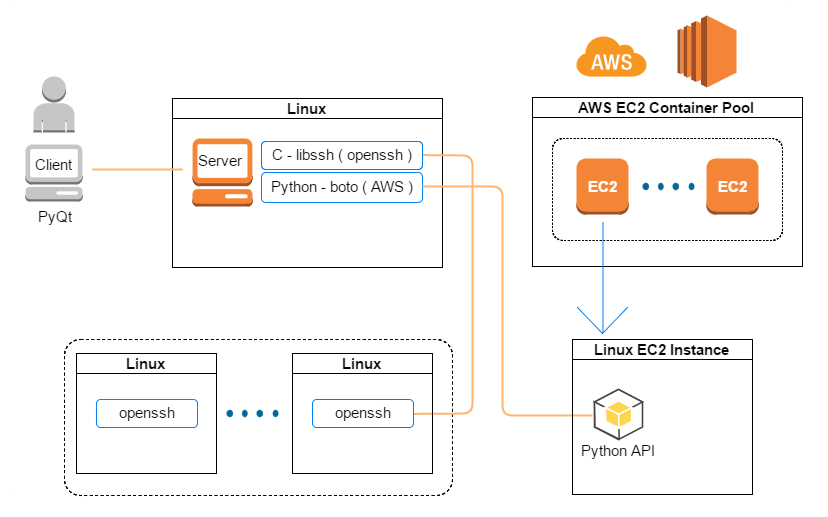
\includegraphics[scale=0.7]{app-layer.png}
\centering
\caption{Application Layer architecture}
\end{figure}

The application flow is:
\begin{itemize}
  \item cloud provider (especially IaaS) agnostic (offering support for Google Cloud Platform and/or Microsoft Azure)
  \item forking the server and hosting it in different geographical locations and infrastructure backbones - for availability / legal reasons
  \item 
\end{itemize}

%
\section{Implementation details}
%
(cod relevant, comentat; use-case-uri)
%
\section{Conclusions}
%
(e.g. cum ar putea fi imbunatatita solutia propusa? )\\
\\

The solution could be extended to be: 

\begin{itemize}
  \item cloud provider (especially IaaS) agnostic (offering support for Google Cloud Platform and/or Microsoft Azure)
  \item forking the server and hosting it in different geographical locations and infrastructure backbones - for availability / legal reasons
  \item 
\end{itemize}

.
%
\\
\\
\\
Solution will be made available at the following address:
 \begin{center}\url{https://github.com/xR86/rc-project}\end{center}

\end{document}
